% This is a model template for the solutions in computational science. You can find a very useful documentation for LaTeX in Finnish at ftp://ftp.funet.fi/pub/TeX/CTAN/info/lshort/finnish/ or in English at ftp://ftp.funet.fi/pub/TeX/CTAN/info/lshort/english/. The section List of mathematical symbols in Chapter 3 is especially useful for the typesetting of mathematical formulas.

% Compile the document to PDF by command 'pdflatex model.tex' in the terminal. The command must be run twice for the references in the text to be correct.

\documentclass[twoside]{article}
\usepackage{graphicx}
\usepackage{lipsum} % Package to generate dummy text throughout this template

\usepackage[sc]{mathpazo} % Use the Palatino font
\usepackage[T1]{fontenc} % Use 8-bit encoding that has 256 glyphs
\linespread{1.05} % Line spacing - Palatino needs more space between lines
\usepackage{microtype} % Slightly tweak font spacing for aesthetics

\usepackage[hmarginratio=1:1,top=32mm,columnsep=20pt]{geometry} % Document margins
\usepackage{multicol} % Used for the two-column layout of the document
\usepackage[hang, small,labelfont=bf,up,textfont=it,up]{caption} % Custom captions under/above floats in tables or figures
\usepackage{booktabs} % Horizontal rules in tables
\usepackage{float} % Required for tables and figures in the multi-column environment - they need to be placed in specific locations with the [H] (e.g. \begin{table}[H])
\usepackage{hyperref} % For hyperlinks in the PDF
\usepackage[english]{babel}
\usepackage{lettrine} % The lettrine is the first enlarged letter at the beginning of the text
\usepackage{paralist} % Used for the compactitem environment which makes bullet points with less space between them
\usepackage{longtable}

\usepackage{abstract} % Allows abstract customization
\renewcommand{\abstractnamefont}{\normalfont\bfseries} % Set the "Abstract" text to bold
\renewcommand{\abstracttextfont}{\normalfont\small\itshape} % Set the abstract itself to small italic text

\usepackage{titlesec} % Allows customization of titles
\renewcommand\thesection{\Roman{section}} % Roman numerals for the sections
\renewcommand\thesubsection{\Roman{subsection}} % Roman numerals for subsections
\titleformat{\section}[block]{\large\scshape\centering}{\thesection.}{1em}{} % Change the look of the section titles
\titleformat{\subsection}[block]{\large}{\thesubsection.}{1em}{} % Change the look of the section titles

\usepackage{fancyhdr} % Headers and footers
\pagestyle{fancy} % All pages have headers and footers
\fancyhead{} % Blank out the default header
\fancyfoot{} % Blank out the default footer
\fancyhead[C]{AS-0.3200 Automaatio- ja systeemitekniikan projektity\"ot} % Custom header text
\fancyfoot[RO,LE]{\thepage} % Custom footer text

%----------------------------------------------------------------------------------------
%	TITLE SECTION
%----------------------------------------------------------------------------------------

\title{\vspace{-15mm}\fontsize{24pt}{10pt}\selectfont\textbf{Nature-Inspired Computing (NIC) Methods in Wind Generator Design Project Documentation}} % Article title

\author{
\large
\textsc{Janne Kemppainen \& Eero J\"arviluoma}\\[2mm] % Your name
\normalsize Aalto University School of Electrical Engineering \\ % Your institution
%\normalsize \href{mailto:john@smith.com}{john@smith.com} % Your email address
\vspace{-5mm}
}
\date{}

%----------------------------------------------------------------------------------------

\makeatletter
\newenvironment{tablehere}
  {\def\@captype{table}}
  {}

\newenvironment{figurehere}
  {\def\@captype{figure}}
  {}
\makeatother


\begin{document}

\maketitle % Insert title

\thispagestyle{fancy} % All pages have headers and footers

%----------------------------------------------------------------------------------------
%	ABSTRACT
%----------------------------------------------------------------------------------------

\begin{abstract}

\noindent This document is the documentation for the project Nature-Inspired Computing (NIC) Methods in Wind Generator Design for the course AS-0.3200 Automaatio- ja systeemitekniikan projektity\"ot. NIC methods include various different algorithms for efficiently finding near-optimal solutions for many optimizing problems.

\end{abstract}

%----------------------------------------------------------------------------------------
%	ARTICLE CONTENTS
%----------------------------------------------------------------------------------------

\begin{multicols}{2} % Two-column layout throughout the main article text

\section{The Goal}

\lettrine[nindent=0em,lines=3]{T}{he} goal of this project is to implement two nature-inspired algorithms for optimizing wind generator design. The generator design module is provided by VTT and it is handled as a black box. The methods used in this project are Genetic Algorithms (GA) and Particle Swarm Optimization (PSO). We describe the basics of the algorithms, our implementations and the findings.

At the end of this project we should atleast have ready implementations for both of the algorithms for optimization of one objective. Depending on the workload and difficulty of implementation multiobjective optimization is also considered.

The aim for the workload was 4cr which equals approximately 100 hours.

We acknowledge the computational resources provided by Aalto Science-IT project.




%------------------------------------------------

\section{The Optimization Problem}
Our optimization problem is a black box model of a wind turbine generator developed by VTT. The model has 14 inputs and 6 outputs. Two of the inputs are integer values and the rest are floating point numbers. In addition to this there are 3 constraints that should be met for the design. 
	
An ideal generator would produce 3 MW of power and have a maximised torque density, minimum weight, high efficiency, high power factor and minimised costs. All the goals can't be optimised simultaneously as they require different parameter combinations. The optimal solution is a compromise where improving some value would deteriorate the others.

For the constraints $\tau_u$ should be at least 7 mm, the output power should be greater than the target power and the temperature of the permanent magnets should stay below $100\,^{\circ}\mathrm{C}$. If any one of these constraints is violated the generator design should be considered invalid.
%------------------------------------------------

\section{Particle Swarm Optimization}

Implementing the Particle Swarm Optimization algorithm was assigned to Janne. The algorithm was first proposed by James Kennedy and Russel Eberhart in 1995 and in our project is their version of the algorithm is implemented with some minor modifications.

The algorithm itself is quite simple. The solution space is first initialized with particles set to random locations with zero velocity. Then the fitness function is evaluated for each particle and the best coordinates are stored. Then the velocities are calculated with the following formula: \cite{pso}
\begin{verbatim}
vx[][]=vx[][]+
 2*rand()*(pbestx[][]-presentx[][])+
 2*rand()*(pbestx[][gbest]-presentx[][])
\end{verbatim}
	
The positions and velocities are updated until a set criterion is fulfilled. The velocity function has a constant 2 for the stochastic part so that the particles would have the possibility to move over the previous best value. This value yields the best results as there is no good way to individually guess which one of the velocity increments should be weighted more. \cite{pso} 
	
	Our optimization problem is a hybrid of discrete and continuous parameters whereas the original algorithm was developed for continuous case only. Therefore we have to make some special arrangements for the two discrete parameters. Pole pair number is an integer between 20 and 80. The first idea was to approximate handle this parameter as continuous and always round the result. The number of slots per pole per pahse has the possible values of 1, 2 and 3 so the idea was to calculate the optimization for each of the three possible parameter values.
	
	In the implementation it was decided, however, that in the eyes of the algorithm itself all the parameters would be continous. The simulation model doesn't allow for non-integer parameters so before each run the corresponding values are rounded to the nearest integer before running the model.
	
	The implementation began with defining the required variables for the swarm and the limitations. The easy part was to fill the solution space with random particles. After implementing the basic algorithm some problems emerged.
	
	The first disturbing observation was that the computer resources weren't used to their full potential as the calculations were performed mostly on one core at a time. After some research the Matlab Parallel Computing Toolbox, and especially the parfor loop, was found. This allowed for the parallelization of the generator simulation and somewhat improved the performance. Not everything is parallelizable though as the particles have to be synchronized. 
	
	The next problem was how to enforce the modeling limitations. The initial attempt was to enforce the parameters to stay inside the defined problem space but this is against the nature of the algorithm. As a result the particles would often hit the hard limits and gather near the edges. The decision was made to check the boundaries but skip the calculations and assign a bad fitness value if any of the parameters were out of bounds.
	
	After the change in handling the boundaries it was noticed that the swarm diverges for some reason. In spite of penalizing out of bounds values the particles seemed to wander far from the desired area. This had to be looked into.
	
	After finding the document by Engelbrecht ~\cite{pitfalls} it became evident that the particle velocities exploded. Using a simpler model $f(x,y)=-x^2-y^2$ yielded similar results, so the next step was to introduce velocity clamping. By changing the fraction of the maximum allowed velocity related to the size of the parameter space it is possible to adjust the particle convergence speed and the tendency of the particles wandering off.
	
	There was also the fundamental mistake that the best particle index was not updated properly so the best value remained to be the one that happened to be the best one on the initialization. This was observed as one of the particles would not move at all.

	Running the provided simulation model was inconsistent performance wise. Usually the simulation was calculated in much less than one second but sometimes the calculation could take several seconds, though. This might happen because of nearly singular matrices in the model but the issue is out of our reach.

	To manage the large amount of computations in a reasonable time we chose to take advantage of the Aalto University Triton computing cluster. The usage of Triton is described in its own chapter.

\section{Genetic Algorithm}

	Genetic Algorithm was implemented by Eero. The algorithm is modeled from Darwin's theory of evolution. A good overview and discussion on the genetic algorithm is presented in ~\cite{mitchell}. In terms of actual implementation, the Genetic Algorithm is based on 5 different steps ~\cite{obitko}:
	\begin{enumerate} \itemsep1pt \parskip0pt \parsep0pt
	\item New Population
	\item Fitness evaluation
	\item Creating a new population
	\item Looping from step 2.
	\end{enumerate}
 	
	In step 1, a random new population is generated.  Population size may vary, but a too large population will lead to unacceptable waste of calculating time and offers very little in return when compared to smaller population sizes. A good population size is around 20-40 candidates.


	In step 2, the fitness of each candidate is evaluated.  Fitness describes how well the candidate satisfies our criteria.Our fitness evaluation is based on the simulation model provided to us by VTT.
	
	In step 3 a new population is created. First, 10 survivals are  selected based on "pie chart roulette", that is, most fit candidates are most likely to survive, but the process is also based on randomness. Next, the survivals produce offspring, and stand a chance to create corssovers with each other. This means that the survivals' offspring inherit attributes from both parents. The best candidate is passed on to the next generation as is. This is called elitism. Finally, a  random, low-chance, mutation may occur. In our case this means that a random parameter  of a random  candidate will be incremented or decremented by a small amount.
	
	The methods used in step 3 and how often they occur are based on empirical evidence. Good  chance for crossover is determined to be around 0.7, for example. Mutation chance needs to be low, or else the process loses it's properties and becomes essentially a random-walk process. However, a low mutation chance is required to make the system evolve.
	
	The simulation results show that the used genetic algorithm managed to find a reasonable good result in practical timeframe. However, the algorithm suffered from 2 drawbacks. Firstly, the algorithm was quite slow when compared to the PSO algorithm. This is probably due to selection process, which requires multiple for-loops at each iteration. Additionally, parallel for loops were not used in the GA code, so the performance could probably have been improved without influencing the overall functionality of the algorithm. The cluster computations were performed with a single core assigned to each task so the performance is comparable in that regard, though. All in all, with the given simulation model, the PSO was almost 10 times faster than GA.
	
	The second drawback with GA was that the solutions weren't quite as good as the ones found by PSO. We are quite sure this had to do with the roulette-wheel selection used in GA. If the fitness values of 2 diffirent candidates are very close to each other, say 0.978 and 0.977, the diffirence in fitness is negligible and the randomness of the "roulette-wheel" takes over. What happens is the solutions become basicly a random-walk process as long as the fitness values don't significantly differ from each other. Therefore the algorithm with this selection method is poorly suited for high end optimization and fine tuning. We could have tested diffirent selection methods, but didn't have time to implement them in the scope of this project work.
	
	
	\section{Computing in the Cluster}
	The calculation capabilities of the home computers proved to be inadequate when we decided to run multiple iterations of the algorithms so that we could investigate the consistency of the results. For example running the PSO algorithm with a swarm size of 50 and 150 simulation time steps took several hours to produce 70 results. The performance felt insufficient so we chose to search for alternative methods.
	
	The next attempt was to try to utilize the new Aalto servers Brute and Force. However, their Matlab license allows only for 12 parallel workers and as the server CPU cores run only at a bit over 2 GHz the performance was very similar to the home computer.
	
	Disappointed with the performance of the available resources we came upon the Aalto Triton computing cluster. Running some 400 compute nodes it was even more than we were looking for. The cluster is in constant heavy use by other researchers so naturally we couldn't use all the possible resources although there was no need for that either.
	
	The cluster is running Scientific Linux and the computation tasks are delivered as batch jobs. We had to adapt the Matlab scripts to the requirements of the environment. The algorithms run as functions that among other parameters take the batch ID so that the computation results can be stored to different files. The batch system runs multiple instances of Matlab on different compute nodes simultaneously. 
	
		We mainly used the 4 hour limit for our batch jobs as it was the maximum time setting for the task to be assigned to the short partition of the cluster. In the short partition we had a better chance of getting the recources quickly when compared to the main partition. Also the 4 hour limit with a one hour grace period was enough for most runs of the PSO algorithm with 10 000 iterations.
	
	After the calculations the saved .mat files are transferred for further analysis. A script reads the output files one by one and then analyzes the results.
	
	
	
\section{Analyzing the Results}
We performed many and more calculations which to analyze. For each algorithm we selected the goal of 10,000 iterations as a baseline. The time allocated for the task was four hours with a grace period of approximately one hour. In the analysis we only used the base versions of the algorithms. 

As noted previously, we only considered the single goal optimization problem of the efficiency. A more practical result could be achieved if the optimization goal was altered in a way that the other generator properties are taken into account. Initially, we tried this approach by setting certain weights to the parameters but the results didn't have any real meaning and they weren't very easy to interpret. 

The final results of the simulations are shown in Appendix A. The results show that the 2 algorithms find their solutions in roughly the same areas. Due to GA's mutation element, the results found by GA are much more spread out when compared to PSO. As mentioned earlier, the GA turns basicly into a random walk process with parameters that don't have a major impact on the fitness. This is especially obvious with parameters 13 and 14, which seem to have very little impact on the generator efficiency.

A better way of doing this multiple goal optimization could be setting some restrictions to the desired properties. As was seen in the comparison of the best generators (Appendix A, Table 1) the one that we got from the PSO algorithm was almost twice the price of the GA version. We could simultaneously optimize the generator efficiency and the power factor by simply taking the sum of these properties. For the other parameters we could set some desired conditions that should be fulfilled and give some penalty if the limits are exceeded. For example, we could set the maximum allowed cost to be 7M and the minimum torque density to 11. We did not have the time to implement this.



\section{Conclusions and Further Research}

Here in our project the PSO algorithm outperformed the genetic algorithm in speed even with a larger swarm than the GA population. Also the achieved fitness value was better. This doesn't necessarily mean that the algorithm itself is any worse but perhaps the scripts weren't equally optimized perfomance and parameter wise.

The next step would be to try to improve the performance of the genetic algorithm by trying to get rid of as many for-loops as possible. Where possible, the PSO implementation already makes use of the Matlab matrix operations which are proved to be more efficcient when compared to the for-loop. After this a better optimization goal should be formed such that every goal would be optimized in a way. A more advanced approach would be to try to achieve Pareto optimality.

\section{Time and Teamwork Management}
The initial project plan had quite amibitous goals for the time management. Due to many reasons they were delayed to the official course deadlines. For example in March and April the project was on halt for almost 4 weeks because of other more urgent assignments.

The workload wasn't evenly distributed because Janne handled the cluster computing in addition to his own algorithm design. Also the available data had to be analyzed so that the feasibility of the results could be verified. This analysis later became the core of the achieved results. Otherwise there were no problems distributing the work as the algorithms required approximately the same amount of work. We could have spent much more time improving both algorithms, but had to keep the time spent on reasonable levels, keeping the scope of the project in mind.

The overall time usage for Janne was 109 hours and 77.5 hours for Eero. These are conservative estimates, as not every task was included in the calculations and some tasks probably took a bit longer than was reported. The time usage can be seen in more detail in Appendix B.



\begin{thebibliography}{99} % Bibliography - this is intentionally simple in this template
\bibitem{pso}
 Kennedy, J. and Eberhart, R.
  \emph{Particle Swarm Optimization},
 Proceedings of IEEE international conference on neural networks. Vol. 4. No. 2. 1995. 

\bibitem{pitfalls}
 Engelbrecht, A. \emph{Particle Swarm Optimization: Pitfalls and Convergence Aspects.}
 Department of Computer Science, University of Pretoria, South Africa
 
\bibitem{mitchell}
Mitchell, M. \emph{An Introduction to Genetic Algorithms.} First MIT paperback edition, fifth printing, 1999. 
 
\bibitem{obitko}
Obitko, M., \emph{Introduction to genetic algorithms}, Hochschule f\"ur Technik und Wirtschaft Dresden (FH), \url{http://www.obitko.com/tutorials/genetic-algorithms/index.php}, accessed 3.3.2014

\end{thebibliography}


\end{multicols}
\newpage
\appendix
\section{Result comparison}
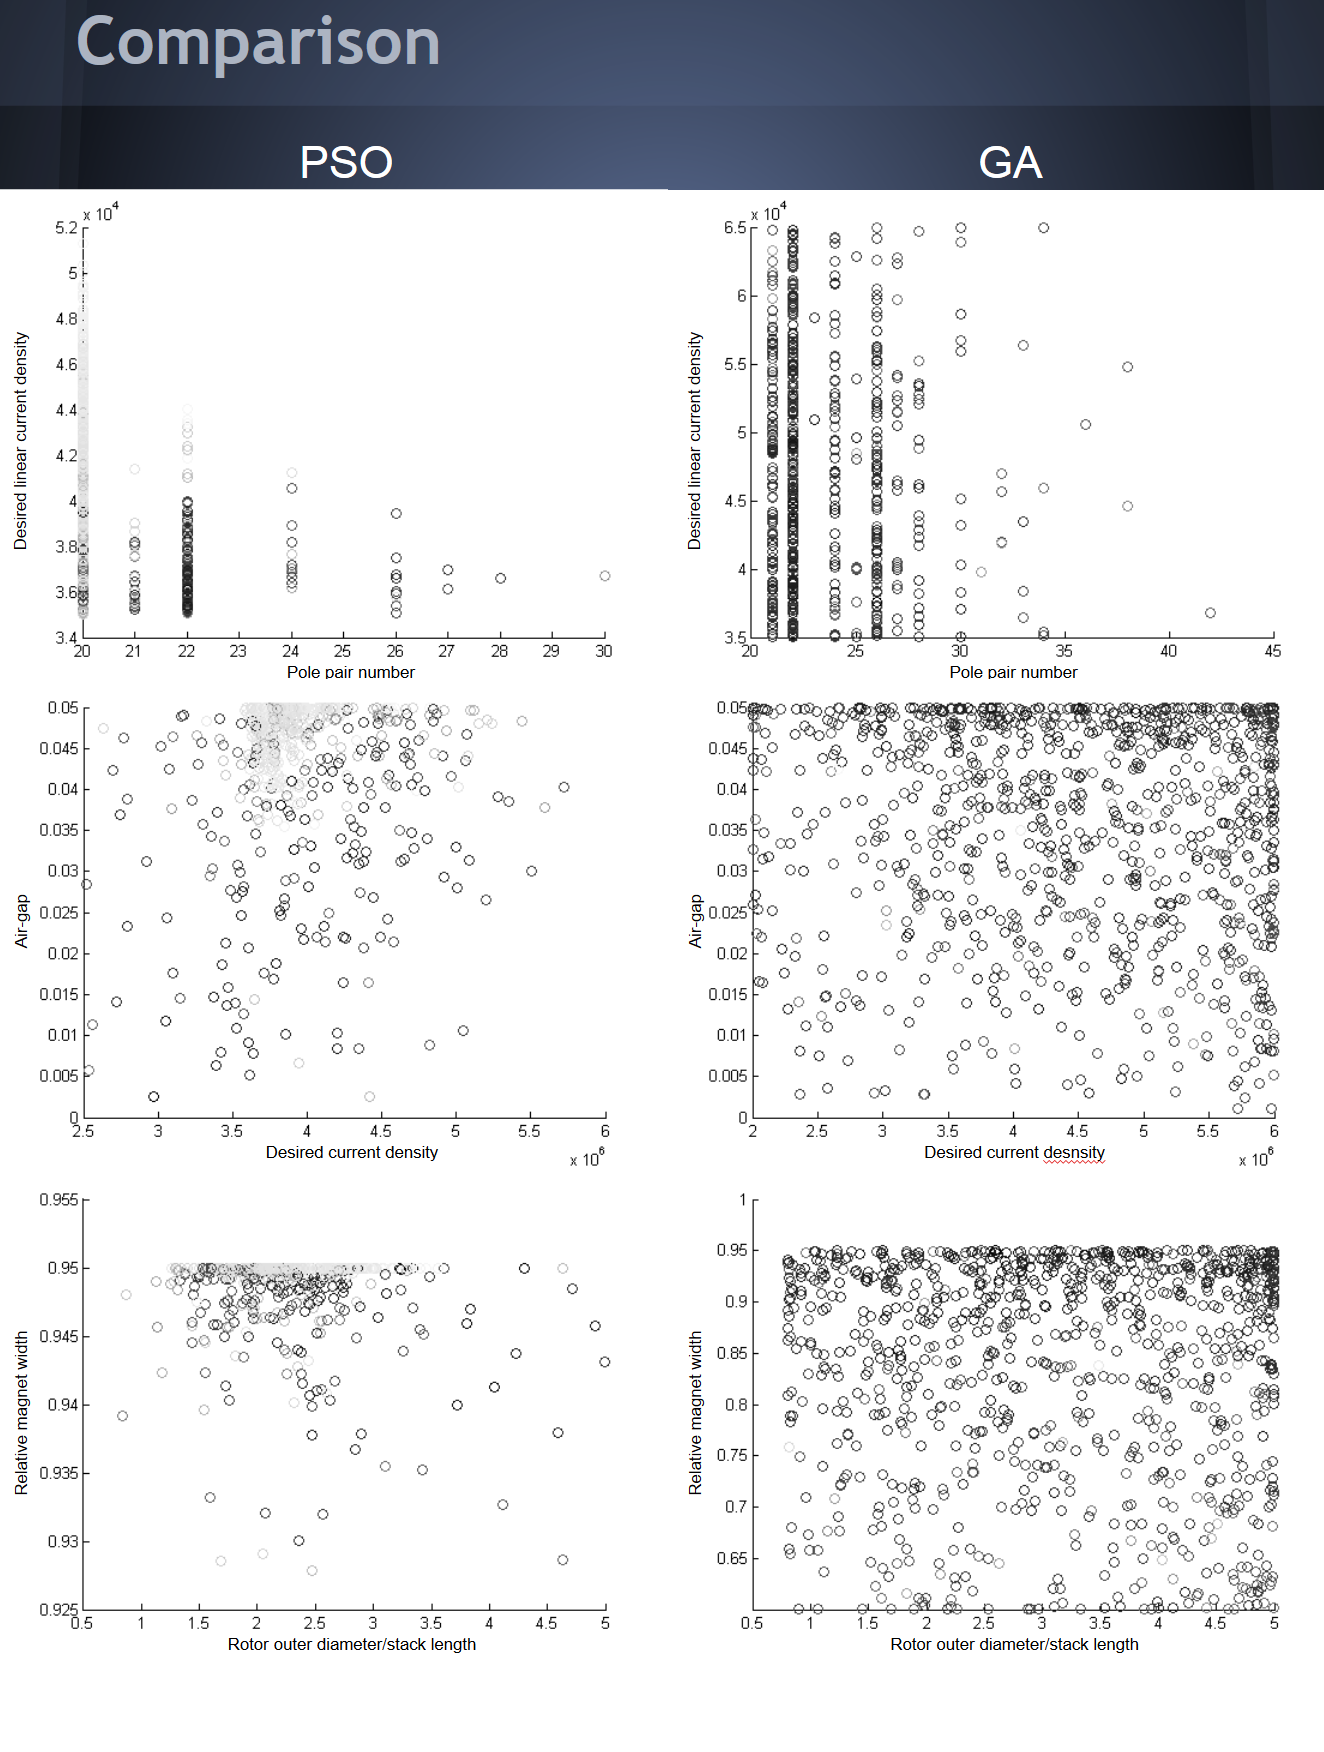
\includegraphics[width=\textwidth,height=\textheight,keepaspectratio]{results1.png}
\newpage
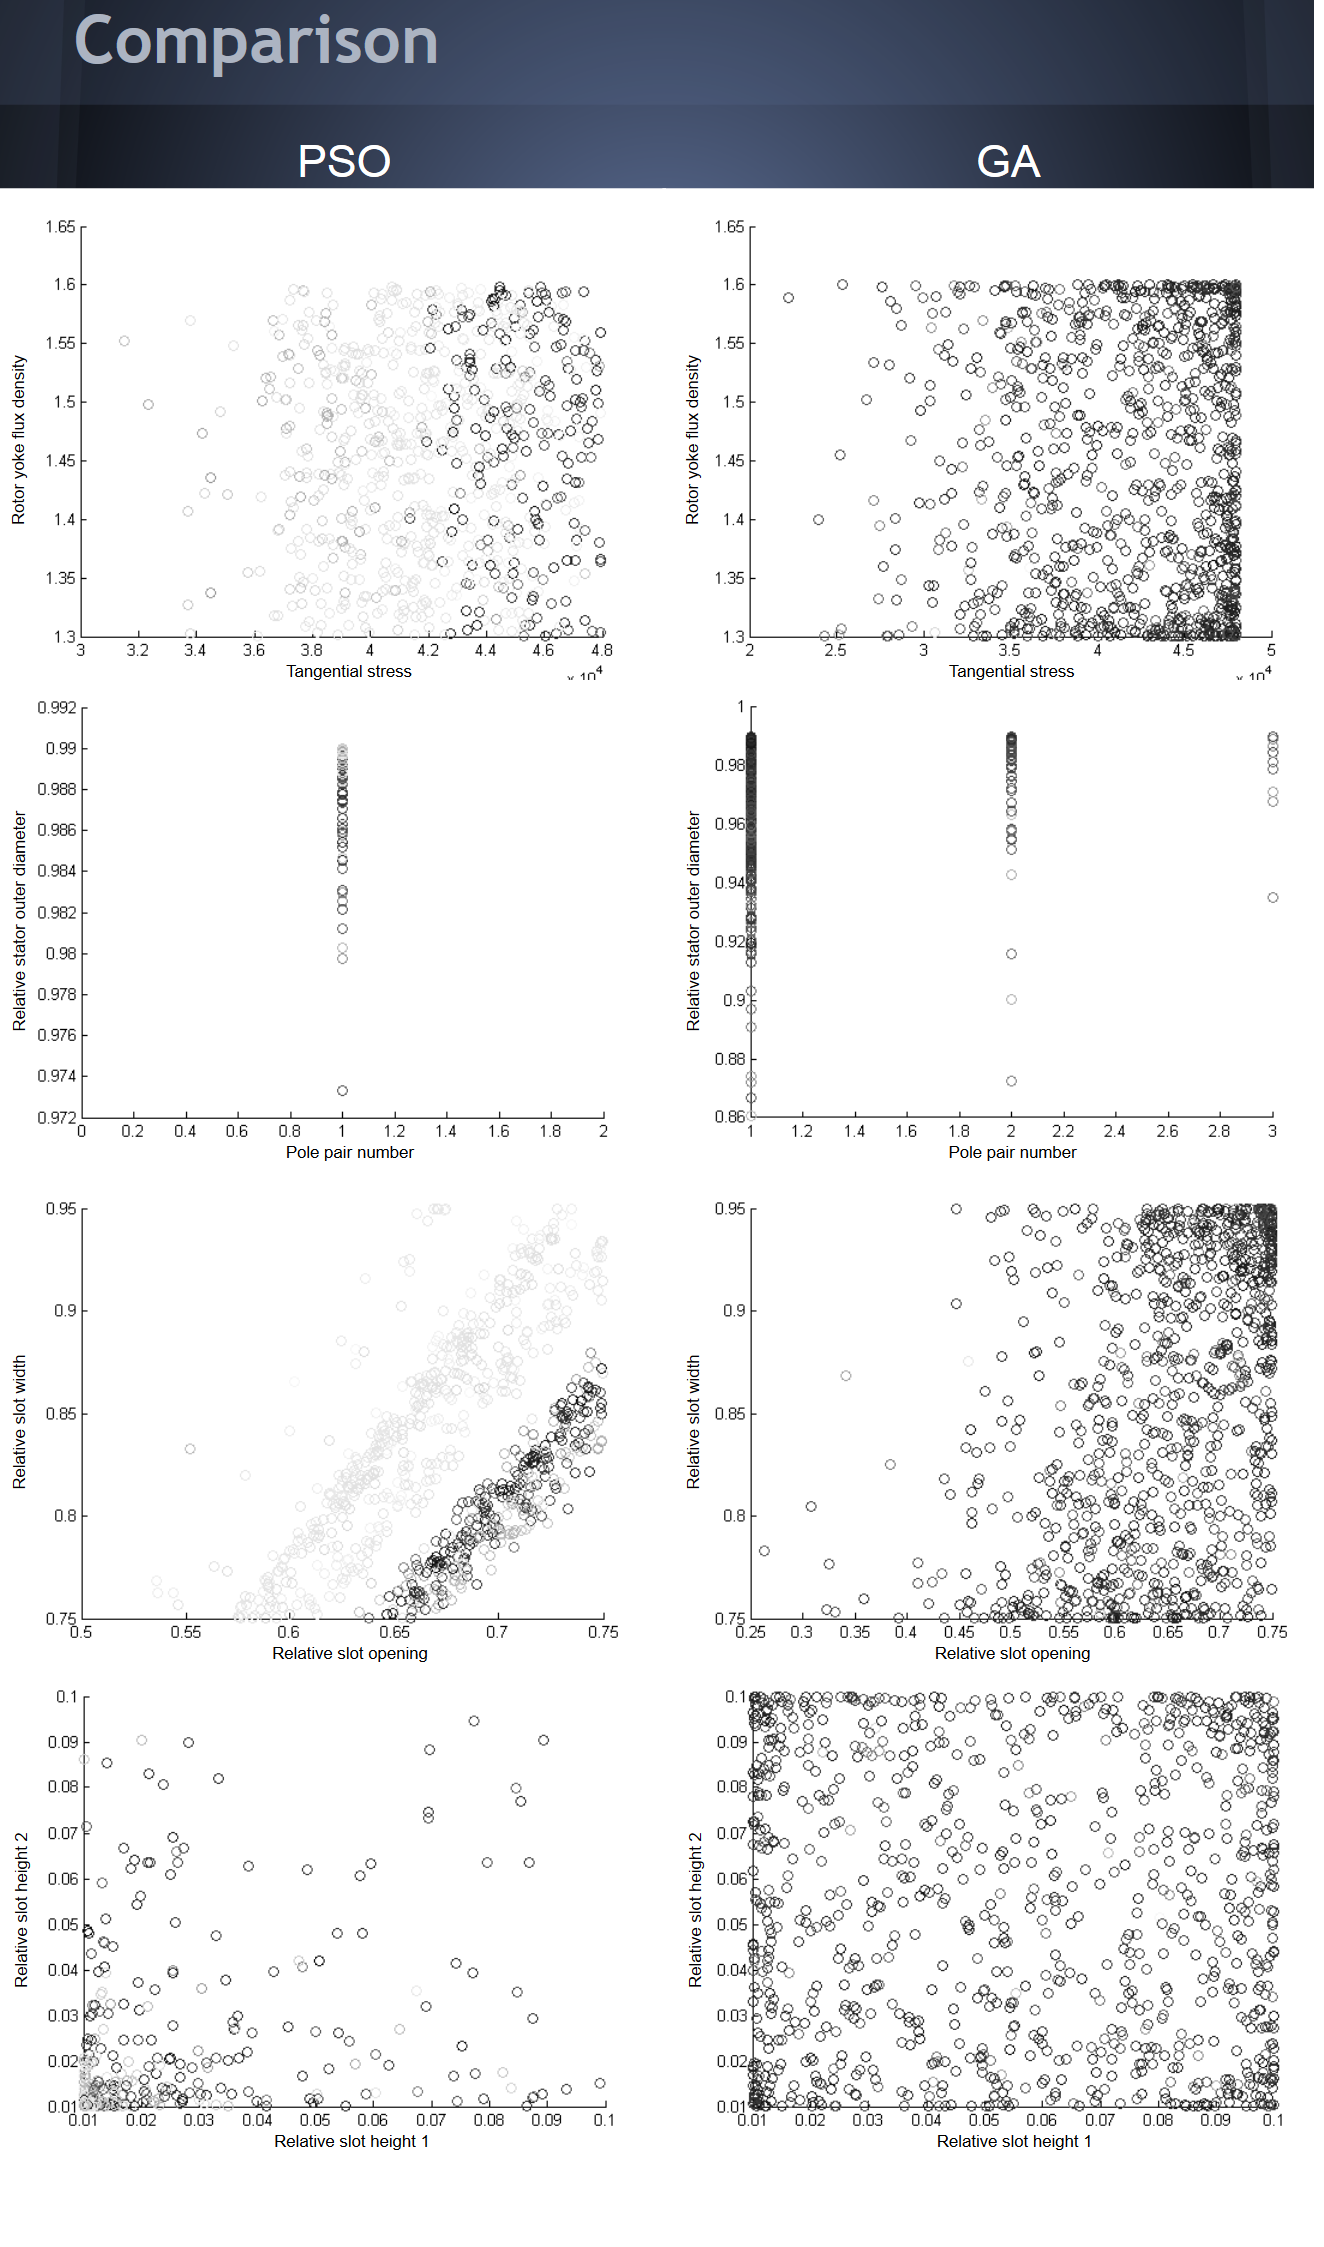
\includegraphics[width=\textwidth,height=\textheight,keepaspectratio]{results2.png}
\newpage
\centering
\begin{table}
\caption{Comparison of the best generators}
\centering
\begin{tabular}{  l  l  l  }

	 & PSO & GA \\ \hline
	Output power (3MW) & 3.0107 MW & 3.0625 MW \\ 
	Torque density & 1475489 & 2513175 \\ 
	Mass & 1.6159e+05 & 1.4712+05 \\ 
	Efficiency & 0.9891 & 0.9856 \\ 
	Power factor & 0.9966 & 0.8206 \\ 
	Cost & 9.0962e+06 & 5.3166e+06 \\ 
\end{tabular}

\end{table}
\clearpage

\section{Time management}
\begin{longtable}{ | l | l | p{10cm} | }
\hline
	lectures & 12 & \  \\ \hline
	\  & \  & \  \\ \hline
	\textbf{Janne} & \textbf{total} & 97 \\ \hline
	\ & \ total + lectures & 109  \\ \hline
	date & time (h) & description \\ \hline
	20.1.2014 & 2 & Familiarization with the project and exploring different algorithms \\ \hline
	21.1.2014 & 1 & Checking the Matlab files \\ \hline
	24.1.2014 & 2 & Project planning \\ \hline
	25.1.2014 & 2.5 & Updating the plan to LaTeX \\ \hline
	30.1.2014 & 0.5 & First meeting \\ \hline
	15.2.2014 & 1 & Reading about the PSO algorithm \\ \hline
	17.2.2014 & 7 & Implementing PSO \\ \hline
	17.2.2014 & 2 & Studying parallelization \\ \hline
	18.2.2014 & 1 & Figuring out performance issues \\ \hline
	24.2.2014 & 4 & Matlab movie capture, wondering why the algorithm doesn't work \\ \hline
	2.3.2014 & 5 & Intermediate report writing \\ \hline
	2.3.2014 & 1.5 & Troubleshooting with simpler algorithm \\ \hline
	3.3.2014 & 1 & Preparing presentation slides \\ \hline
	3.3.2014 & 1 & Velocity clamping \\ \hline
	3.3.2014 & 1 & Finding suitable software to capture video from screen \\ \hline
	4.3.2014 & 1 & Intermediate report writing \\ \hline
	4.3.2014 & 0.5 & Video editing and upload to YouTube \\ \hline
	15.3.2014 & 1 & Started a clean attempt of PSO in order to improve code readability \\ \hline
	15.3.2014 & 1 & How  to apply a function only to a subset of matrix elements \\ \hline
	16.3.2014 & 1 & Wondering one particle immobility \\ \hline
	16.3.2014 & 1 & Found the reason for the problem, there was a typo in the bestidx parameter \\ \hline
	17.3.2014 & 3 & Improve plotting, run simulation with large swarm, parametrize velocity calculation \\ \hline
	17.3.2014 & 1 & Print text to console, run multiple simulations \\ \hline
	18.3.2014 & 1 & Explore multidimensional data visualization \\ \hline
	19.3.2014 & 2 & Gather data for multiple runs of PSO \\ \hline
	22.3.2014 & 1 & Found out that the data from the 5 hour run was not saved. Started new calculation runs. \\ \hline
	23.3.2014 & 1.5 & Write script to analyze the optimal parameter distributions. Find info about the computing facilities in Aalto. \\ \hline
	23.3.2014 & 0.5 & Apply for a Triton account. \\ \hline
	23.3.2014 & 1 & Reading about various inertia handling methods. \\ \hline
	24.3.2014 & 1 & Ask for Triton account, discuss with Eero about the project. \\ \hline
	25.3.2014 & 1.5 & Read Triton manuals and about Bash scripting \\ \hline
	26.3.2014 & 1.5 & Read about SLURM and sbatch, project discussion \\ \hline
	26.3.2014 & 1.5 & Implementing PSO to be used in Triton \\ \hline
	26.3.2014 & 1.5 & Experiment with Bash scripting, script .mat file upload from Triton to Kosh \\ \hline
	26.3.2014 & 1 & Run tests and benchmark on home computer. Run hundred iterations on cluster. \\ \hline
	26.3.2014 & 1 & Every calculation produced the same results, set the random number seed manually. Start new calculation with 200 tasks. \\ \hline
	27.3.2014 & 0.5 & Basic analyzation of the data. \\ \hline
	22.4.2014 & 0.5 & Telling Eero what kind of function he should make so that it could be run in Triton, fixed random number generation \\ \hline
	23.4.2014 & 2 & Documentation \\ \hline
	23.4.2014 & 0.5 & For some reason the PSO\_SLURM folder was deleted. Recovered missing files. \\ \hline
	24.4.2014 & 0.5 & Fixed documentation \\ \hline
	24.4.2014 & 1.5 & Run simulations for random inertia \\ \hline
	25.4.2014 & 1 & Some shell wizardry to find the failed (old) results and remove them as I forgot to clean the folder before running the job \\ \hline
	26.4.2014 & 1 & What to do with the data and is the collected data sufficient? \\ \hline
	26.4.2014 & 0.5 & Set up SSH tunneling so that the file transfering is easier \\ \hline
	26.4.2014 & 1 & Prepare and run new batch jobs \\ \hline
	26.4.2014 & 1 & The previous run was erroneous, made some modifications and started new batch jobs \\ \hline
	27.4.2014 & 0.5 & Check the simulation results \\ \hline
	29.4.2014 & 1 & Lunch discussion with Eero about the \\ \hline
	29.4.2014 & 0.5 & Write e-mail \\ \hline
	29.4.2014 & 1 & Prepare and run the GA simulations \\ \hline
	2.5.2014 & 2 & Change the fitness function to efficiency only, remove the saving of the development of the swarm from PSO\_function, test, start new calculation in cluster \\ \hline
	2.5.2014 & 2 & Checking results and plotting plots \\ \hline
	9.5.2014 & 1 & Prepare and run GA with updated fitness function \\ \hline
	9.5.2014 & 0.5 & Start making presentation slides \\ \hline
	10.5.2014 & 1 & Changed GA to utilize parfor and started new runs. The previous run had only 1000 iterations and the convergence limit of 200. \\ \hline
	10.5.2014 & 1 & Prepare slides and make changes so that the values are stored to the disk after always after certain amount of iterations instead of at the end. \\ \hline
	10.5.2014 & 1 & Fight with the batch jobs \\ \hline
	10.5.2014 & 1 & Data analysis \\ \hline
	10.5.2014 & 3 & Visualizations and making slides \\ \hline
	10.5.2014 & 0.5 & Check and upload last GA runs \\ \hline
	11.5.2014 & 2 & Fighting with network problems \\ \hline
	11.5.2014 & 3 & Development of PSO fitness visualization \\ \hline
	11.5.2014 & 2 & Prepare slides \\ \hline
	12.5.2014 & 1.5 & Prepare slides \\ \hline
	12.5.2014 & 0.5 & Run GA, then run it again \\ \hline
	22.5.2014 & 2.5 & Documentation \\ \hline
	25.5.2014 & 1.5 & Documentaiton \\ \hline
	

\end{longtable}

\begin{tabular}{|l|l|l|}
\hline
	\textbf{Eero} & \textbf{total} & \textbf{64.5} \\ \hline
	total + lectures & 77.5 & \  \\ \hline
	2.3.2014 & 32 & intermediate report total \\ \hline
	14.3.2014 & 3 & Trouoble with the sum function, calculating fitness \\ \hline
	17.3.2014 & 2 & Fine-tuning the selection process \\ \hline
	17.3.2014 & 2.5 & Fixed a bug with crossover, first working model \\ \hline
	24.3.2014 & 1 & Miscellaneous discussion (including Triton) \\ \hline
	26.3.2014 & 1.5 & Modifying GA to handle negative fitness values \\ \hline
	28.4.2014 & 6 & Huge revamp to reduce convergence to single solution \\ \hline
	29.4.2014 & 1 & Lunch with Janne, discussion about data analysis \\ \hline
	10.5.2014 & 4 & Mutation chance analysis \\ \hline
	11.5.2014 & 6 & Mutation chance analysis, average fitness analysis \\ \hline
	12.5.2014 & 1 & Tweaking mutation chance, one more iteration on Triton \\ \hline
	12.5.2014 & 2.5 & Making slides \\ \hline
	23.5.2014 & 4 & Documentation \\ \hline
\end{tabular}



\end{document}